\PassOptionsToPackage{table}{xcolor}
\documentclass[11pt,twoside]{article}

\usepackage[margin=1in]{geometry}
\usepackage[T1]{fontenc}
\usepackage{lmodern}
\usepackage[utf8]{inputenc}
\usepackage{microtype}
\usepackage{xcolor}
\usepackage{setspace}
\definecolor{headergray}{gray}{0.50}
\definecolor{footgray}{gray}{0.50}
\definecolor{tableheaderbg}{gray}{0.82}
\definecolor{tablerowbg}{gray}{0.94}
\usepackage{amsmath,amssymb,amsthm,mathtools}
\usepackage{enumitem}
\usepackage{booktabs}
\usepackage{array}
\usepackage{caption}
\usepackage{tikz}
\usetikzlibrary{arrows.meta,positioning,calc,fit,backgrounds}
\usepackage[colorlinks=true,linkcolor=blue,citecolor=blue,urlcolor=blue]{hyperref}
\usepackage[nameinlink,noabbrev]{cleveref}
\usepackage{csquotes}
\usepackage[backend=biber,style=alphabetic,sorting=nyt,maxbibnames=99]{biblatex}
\addbibresource{observer_geometry_3.refs.bib}
\usepackage{fancyhdr}
\usepackage{lastpage}
\usepackage{etoolbox}

\hypersetup{
  pdftitle={Observer Geometry III},
  pdfauthor={James Ross},
  pdfpagelayout=SinglePage,
  pdfdirection=L2R
}

% Typography controls for publication-style pagination.
\clubpenalty=10000
\widowpenalty=10000
\displaywidowpenalty=10000
\brokenpenalty=10000
\interfootnotelinepenalty=10000
\doublehyphendemerits=100000
\finalhyphendemerits=1000000
\emergencystretch=2em
\raggedbottom
\setstretch{1.12}
\setlength{\parindent}{0pt}
\setlength{\parskip}{0.72em}

\captionsetup[figure]{font=small,labelfont=bf,textfont=it}
\captionsetup[table]{font={small},labelfont=bf}
\newcommand{\TableHeaderRow}{\rowcolor{tableheaderbg}\bfseries}
\AtBeginEnvironment{table}{\rowcolors{2}{tablerowbg}{white}}
\AtEndEnvironment{table}{\rowcolors{2}{}{}}

\setlength{\headheight}{30pt}
\newcommand{\paperdoi}{Draft manuscript}
\newcommand{\paperversion}{Version 0.1.0-draft}
\newcommand{\publicationdate}{May 2026}
\newcommand{\runningauthor}{James Ross}
\newcommand{\runningtitle}{Observer Geometry III}

\fancypagestyle{ogmain}{%
  \fancyhf{}
  \fancyhead[C]{\footnotesize \textcolor{headergray}{\runningtitle}}
  \fancyfoot[R]{\footnotesize \textcolor{footgray}{\thepage\ of \pageref*{LastPage}}}
  \renewcommand{\headrulewidth}{0pt}
  \renewcommand{\footrulewidth}{0pt}
}

\fancypagestyle{ogtitle}{%
  \fancyhf{}
  \fancyfoot[C]{\tiny Copyright \textcopyright\ 2026 James Ross. Licensed under the \href{https://creativecommons.org/licenses/by/4.0/}{Creative Commons Attribution 4.0 International License}.}
  \fancyfoot[R]{\footnotesize \textcolor{footgray}{\thepage\ of \pageref*{LastPage}}}
  \renewcommand{\headrulewidth}{0pt}
  \renewcommand{\footrulewidth}{0pt}
}

\fancypagestyle{plain}{%
  \fancyhf{}
  \fancyhead[C]{\footnotesize \textcolor{headergray}{\runningtitle}}
  \fancyfoot[R]{\footnotesize \textcolor{footgray}{\thepage\ of \pageref*{LastPage}}}
  \renewcommand{\headrulewidth}{0pt}
  \renewcommand{\footrulewidth}{0pt}
}

\pagestyle{ogmain}

\newtheorem{theorem}{Theorem}[section]
\newtheorem{proposition}[theorem]{Proposition}
\newtheorem{lemma}[theorem]{Lemma}
\newtheorem{corollary}[theorem]{Corollary}
\theoremstyle{definition}
\newtheorem{definition}[theorem]{Definition}
\newtheorem{remark}[theorem]{Remark}

\newcommand{\AION}{AI\ensuremath{\Omega}N}
\newcommand{\Obl}{\mathsf{Obl}}
\newcommand{\Carry}{\mathsf{Carry}}
\newcommand{\Unmet}{\mathsf{Unmet}}
\newcommand{\DeclaredLoss}{\mathsf{DeclaredLoss}}
\newcommand{\Debt}{\mathsf{Debt}}
\newcommand{\Supp}{\mathsf{Supp}}
\newcommand{\CryptSupp}{\mathsf{CryptSupp}}
\newcommand{\CWit}{\mathsf{CWit}}
\newcommand{\PathCert}{\mathsf{PathCert}}
\newcommand{\Extract}{\mathsf{Extract}}
\newcommand{\Sat}{\mathsf{Sat}}
\newcommand{\Admit}{\mathsf{Admit}}
\newcommand{\Just}{\mathsf{Just}}
\newcommand{\Report}{\mathsf{Report}}
\newcommand{\Val}{\mathsf{Val}}
\newcommand{\Def}{\mathsf{Def}}
\newcommand{\Verify}{\mathsf{Verify}}
\newcommand{\Refutes}{\mathsf{refutes}}
\newcommand{\OverReport}{\mathsf{OverReport}}
\newcommand{\Hallucinate}{\mathsf{Hallucinate}}
\newcommand{\FalseReport}{\mathsf{FalseReport}}
\newcommand{\Launder}{\mathsf{Launder}}
\newcommand{\ctx}{\mathsf{ctx}}
\newcommand{\fresh}{\mathsf{fresh}}
\newcommand{\stale}{\mathsf{stale}}
\newcommand{\supported}{\mathsf{supported}}
\newcommand{\underdetermined}{\mathsf{underdetermined}}
\newcommand{\authorityblocked}{\mathsf{authority\_blocked}}
\newcommand{\unverifiable}{\mathsf{unverifiable}}

\newcommand{\paperkeywords}{observer geometry; support obligations; proof-carrying paths; witness holonomy; observer-relative claim status; cryptographic witnesses; audit systems}
\newcommand{\paperabstract}{Observer Geometry I showed that observers cannot be reduced to scalar distance: projection, basis, accumulation, aperture, degeneracy, insufficiency, bias gaps, and signatures all separate. Observer Geometry II showed the distributed consequence: state convergence is not observer convergence, because replicas may agree on visible state while retaining, erasing, transforming, or obstructing different witness surfaces. This paper studies the next obstruction. Endpoint agreement is not support agreement. A claim's justified support-status can depend on the path by which support, authority, freshness, and context are transported. We introduce purpose-indexed support obligations, path-indexed carried-support ledgers, declared loss, witness debt, path certificates, and local report-strength preorders. A claim survives transport only when the path preserves, compresses, verifies, opens, or explicitly declares the loss, blocking, staleness, or redaction of the support required for that claim. We prove finite separation results for witness sensitivity, path-dependent support transport, nonzero witness holonomy, validity/admissibility separation, and support-soundness failure. Cryptographic objects are treated as finite witness surfaces that separate commitment, verification, revelation, authority, freshness, and admission. The result is a support-obligation calculus for recording what state arrived and which claims that path is structurally capable of supporting.}

\tikzset{
  ogbox/.style={draw=black, rounded corners=2pt, line width=0.9pt, fill=white, align=center, inner sep=6pt},
  ogaltbox/.style={draw=black, rounded corners=2pt, line width=0.9pt, fill=white, align=center, inner sep=6pt},
  ogwarnbox/.style={draw=black, rounded corners=2pt, line width=0.9pt, fill=white, align=center, inner sep=6pt},
  ogline/.style={-{Latex[length=2.7mm,width=2mm]}, line width=0.9pt},
  ogthin/.style={-{Latex[length=2mm,width=1.5mm]}, line width=0.7pt}
}

\title{Observer Geometry III\\\large Path Geometry and Support Obligations}
\author{}
\date{}

\begin{document}

\begingroup
\thispagestyle{ogtitle}
\begin{center}
\vspace*{-0.03\textheight}
{\fontsize{28}{32}\selectfont\bfseries\fontseries{bx}\selectfont Observer Geometry III\par}
{\fontsize{24}{28}\selectfont\bfseries\fontseries{bx} Path Geometry and Support Obligations\par}
\vspace{0.20em}
{\Large\bfseries Witness Transport and Observer-Relative Claim Status\par}
\vspace{0.18em}
{\normalsize \paperdoi\\[-0.22em]}
{\normalsize \paperversion\enspace|\enspace\publicationdate\par}
\vspace{0.48em}
{\large James Ross\par}
{\normalsize Independent Researcher\\[-0.14em]}
{\normalsize ORCID: 0009-0006-0025-7801\\[-0.14em]}
{\normalsize \href{mailto:james@flyingrobots.dev}{\texttt{james@flyingrobots.dev}}\par}
\vspace{0.85em}
\begin{minipage}{0.82\textwidth}
\small
\textbf{Abstract.} \paperabstract
\par
\vspace{1.25em}

\textbf{Keywords.} \textit{\paperkeywords}
\end{minipage}
\end{center}
\endgroup

\clearpage
\begingroup
\setstretch{0.96}
\setlength{\parskip}{0pt}
\tableofcontents
\endgroup
\clearpage

\section{Introduction}
\label{sec:introduction}

Consider the audit contrast. Two transport paths deliver the same final document
to the same endpoint observer: \texttt{document text = X}. Along the first path,
the object carries a signed edit receipt, an identity binding, a policy epoch,
and a freshness frontier at which those facts can be checked. Along the second
path, the object carries only the final text after copying, redaction, or
summary. A state-reading observer sees the same document in both cases. An
authorship-audit observer sees different support. The claim ``the document
contains text $X$'' may be responsibly reported along both paths; the claim
``Alice authorised edit $e$'' is responsibly reportable only along the path that
carried admissible provenance and authority support.

This paper takes the path-transport slice of the Observer Geometry program.
OG-I modeled observers as structured systems with projection, basis,
accumulation, aperture, degeneracy, insufficiency floors, bias gaps, and
observer signatures~\cite{ross_og_i_2026}. OG-II developed the distributed case:
replicas may converge in visible state while their observer surfaces remain
different, because witnessed updates, frontiers, suffix transport, policy
closure, provenance, and obstruction structure may be retained or erased
differently along the way~\cite{ross_og_ii_2026}. OG-III uses those interfaces
to study claim support across observer paths. Endpoint agreement fixes a visible
surface. It does not fix which witnesses, receipts, authority metadata,
freshness frontiers, and disclosure constraints survived the route by which that
surface arrived.

The paper is organized around one claim: \textbf{endpoint agreement leaves
support agreement open}. A provenance claim, an absence claim, an authority
claim, a freshness claim, and a state claim impose different support
obligations. A path may carry that support directly, compress it into a receipt,
replace it with a cryptographic proof, bind it for future opening, declare it
redacted, mark it authority-blocked, or lose it entirely. The endpoint
observer's responsible status for the claim is bounded by the support that
survived transport in admissible form.

The central object is a path-indexed support judgement built from
\[
  \Obl_{P}(\varphi,\ctx),\qquad
  \Carry_{\gamma}(\varphi,\ctx),\qquad
  \Val_{\gamma}^{P,\ctx}(\varphi).
\]
Here $\Obl_{P}(\varphi,\ctx)$ is the support obligation imposed by claim
$\varphi$ under purpose $P$ and context $\ctx$; $\Carry_{\gamma}(\varphi,\ctx)$
is the support actually carried, compressed, opened, certified, blocked,
redacted, or declared lost along observer path $\gamma$; and
$\Val_{\gamma}^{P,\ctx}(\varphi)$ is the justified status of $\varphi$ after
transport. A path may preserve enough visible structure to make a claim
discussable while dropping the support required for the reported status of that
claim. That gap is witness debt. Witness debt is structural; dishonesty enters
only when an observer reports as if the debt were discharged.

\paragraph{Support transport.}
OG-III keeps the geometry finite, discrete, and witness-based. Observer paths
are finite chains of translators between structured observers. A translator
preserves the coordinates, witnesses, receipts, authority conditions, and
freshness constraints declared for the task. A path therefore moves state and
transforms support. It may preserve support, compress support, certify support,
redact support, block support, launder support, or create support debt.

Cryptographic witnesses matter here because they make several observer
distinctions mathematically sharp. A hash or authenticated root can commit to a
history without revealing it. A signature can bind authorship, authority, or a
frontier. A commitment can preserve future decidability while leaving present
projection degenerate. An authenticated data structure can transport compact
membership, exclusion, or update witnesses. A compact relational proof can
support a relation over committed structure without transporting the full
structure. A zero-knowledge proof can expand verification aperture while keeping
revelation aperture bounded. A capability or encryption condition can make a
claim authority-blocked rather than false. These primitives are treated as
finite witness surfaces: mechanisms that separate visibility, retained support,
verification, revelation, authority, and freshness.

\paragraph{Contributions.}
The paper contributes four pieces:
\begin{enumerate}[leftmargin=*]
  \item A purpose-indexed support-obligation calculus for claims, contexts,
        statuses, carried support, declared loss, and witness debt.
  \item A path-indexed support-transport model with checkable path certificates
        and extraction from endpoint accumulation into claim-purpose-context
        support ledgers.
  \item A finite separation suite for witness sensitivity, path-dependent
        support transport, nonzero witness holonomy, validity/admissibility
        separation, and support-soundness failure.
  \item A cryptographic witness interpretation that treats commitments,
        signatures, authenticated roots, compact proofs, capabilities, and
        disclosure controls as observer surfaces rather than protocol features
        outside the geometry.
\end{enumerate}

\paragraph{Proof boundary.}
The results below should be read with this boundary in mind. OG-III proves
finite separation and accounting statements about support obligations over
declared observer paths. It does not provide a universal truth procedure, a
global merge law, a smooth connection on a manifold, or a completeness theorem
for all possible evidence. Each result is witnessed by a finite observer graph,
a finite support table, and a declared purpose/context pair. The intended
question is local: given the support a path carried or declared lost, which
claim-status reports are structurally justified?

\paragraph{Scope management.}
OG-III remains structural. It analyzes false, unsupported, stale, blocked,
laundered, and overstrong reports as support-status mismatches. It does not
assign dishonesty, culpability, accountability, or rights. Those require a
further theory of reporting obligations: what the observer knew, what it was
entitled to reveal, what it was required to declare, and whether it represented
its support situation accurately. That is the subject of OG-IV. The handoff is
simple: OG-III asks what support exists, survives, verifies, is blocked, is
stale, or is lost; OG-IV asks what the observer claimed about that support, and
whether that claim was honest.

\paragraph{Roadmap.}
Section~\ref{sec:imports} fixes the imported interfaces from OG-I and OG-II.
Section~\ref{sec:claims-obligations} defines claims, support contexts,
statuses, support obligations, carried support, declared loss, and witness debt.
Section~\ref{sec:paths} develops observer paths, path certificates,
satisfaction, admission, and noncommutative support transport.
Section~\ref{sec:path-dependent} proves witness sensitivity and
path-dependent support transport. Section~\ref{sec:crypto} isolates
cryptographic witness surfaces and the verification/admission split.
Section~\ref{sec:holonomy} develops witness holonomy, freshness, and negative
witnesses. Section~\ref{sec:soundness} defines support soundness, overreporting,
hallucination as supported-claim overreport, witness debt, and typed false
reports. Sections~\ref{sec:robustness}--\ref{sec:ogiv} record purpose-indexed
equivalence, engineering implications, and the bridge to OG-IV.

\paragraph{Imported interfaces.}
OG-III imports OG-I and OG-II as fixed public interfaces rather than rederiving
them. From OG-I it uses structural observers, projection, basis, accumulation,
aperture, degeneracy, insufficiency, and observer signatures. From OG-II it uses
frontier-indexed replica observers, witnessed updates, frontiers, suffix
transport, state convergence, and the discipline that visible-state agreement
can leave other observer surfaces separated. In this paper, those interfaces are
reused to ask which claims a transported object can still support.

\paragraph{Self-contained scope.}
For a self-contained reading of OG-III, a reader may take OG-I's observer as an
ordinary structured observation system and OG-II's path language as a finite
transport graph between such systems. Assume deterministic replayable histories,
finite observers, declared purposes, declared support contexts, and checkable
path certificates. Under those assumptions, every new primitive used below is
defined in this paper: support obligations, carried support ledgers, declared
loss, witness debt, satisfaction, admission, path certificates, witness
holonomy, verification/admission separation, and support-soundness failure.

\section{Imported Interfaces from OG-I and OG-II}
\label{sec:imports}

OG-III treats OG-I and OG-II as fixed public interfaces and imports the following terms without re-teaching either paper.

\begin{table}[ht]
\centering
\small
\begin{tabular}{p{0.19\textwidth}p{0.11\textwidth}p{0.31\textwidth}p{0.27\textwidth}}
\toprule
\TableHeaderRow Term & Source & Imported meaning & OG-III use \\
\midrule
Observer & OG-I & Structured observer, not scalar point & Endpoint or node of support transport \\
Projection & OG-I & Visible state under observer aperture & Endpoint equality condition \\
Basis & OG-I & Representational coordinate frame & Claim/status interpretation \\
Accumulation & OG-I & Observer memory/update state & Source for $\Extract(\cdots M_S \cdots)$ \\
Aperture & OG-I & What can be observed, retained, checked, or revealed & Support and revelation limits \\
Degeneracy & OG-I & Distinct histories collapse to same projection & Source of witness sensitivity \\
Replica observer & OG-II & Frontier-indexed distributed observer & Source of path/worldline examples \\
Witnessed update & OG-II & Update with retained support surface & Raw material for $\Carry_\gamma$ \\
Frontier & OG-II & Causal, log, policy, or freshness boundary & Freshness and negative witnesses \\
Suffix transport & OG-II & Transport of witnessed suffixes & Precursor to proof-carrying paths \\
State convergence & OG-II & Endpoint visible state agreement & Explicitly not support agreement \\
\bottomrule
\end{tabular}
\caption{Minimal imported glossary. Full glossary and notation concordance appear in \cref{app:glossary}.}
\label{tab:imported-glossary}
\end{table}

\section{Claims, Contexts, Statuses, and Support Obligations}
\label{sec:claims-obligations}

\begin{definition}[Support context]
A support context records the purpose and local admissibility frame under which a claim is evaluated:
\[
  \ctx_{\mathrm{base}}=(P,F,\alpha,\mathrm{disclosure},\mathrm{expiry}).
\]
Once a transport path is fixed, OG-III writes $\ctx_\gamma=(\ctx_{\mathrm{base}},\gamma)$.
\end{definition}

\begin{definition}[Support obligation]
For a claim $\phi$, purpose $P$, and context $\ctx$, the support obligation
\[
  \Obl_P(\phi,\ctx)
\]
is the finite set or typed structure of support coordinates required to responsibly report $\phi$ for $P$ in $\ctx$. Obligations may require state, provenance, intent, authority, negative witness, frontier/freshness, verification, revelation, or admission-policy support.
\end{definition}

\begin{definition}[Status discipline]
Statuses are finite tags, not a global truth lattice. OG-III uses tags such as
\[
  \supported,\quad \underdetermined,\quad \authorityblocked,\quad \unverifiable,\quad \stale
\]
to name different support situations. The report-strength preorder introduced in
\cref{sec:soundness} is local to a purpose $P$ and context $\ctx$. In
particular, $\authorityblocked$, $\underdetermined$, and $\unverifiable$ are not
globally ordered; each names a different obstruction to responsible reporting.
\end{definition}

\begin{table}[ht]
\centering
\small
\begin{tabular}{>{\raggedright\arraybackslash}p{0.25\textwidth}>{\raggedright\arraybackslash}p{0.18\textwidth}>{\raggedright\arraybackslash}p{0.45\textwidth}}
\toprule
\TableHeaderRow Claim & Purpose & Typical required support \\
\midrule
\enquote{document contains text $X$} & reading & endpoint projection and relevant state root \\
\enquote{Alice authorised edit $e$} & authorship audit & signature, identity binding, policy epoch, and path certificate \\
\enquote{key $k$ was not revoked at frontier $F$} & non-revocation & log frontier, non-membership witness, consistency relation, and freshness proof \\
\enquote{predicate $Q(x)$ holds} & sealed verification & commitment, public inputs, proof object, and context binding \\
\enquote{$L$ reported $\phi$} & testimony audit & report provenance, speaker identity, utterance context, and path from $L$ to $S$ \\
\bottomrule
\end{tabular}
\caption{Finite support-obligation sketches. $\Obl_P(\phi,\ctx)$ changes with the claim family, purpose, and context.}
\label{tab:obligation-sketches}
\end{table}

\begin{proposition}[Testimony/Object Claim Separation]
Let $\psi_L(\phi)$ denote the testimony claim \enquote{$L$ reported $\phi$}.
In general,
\[
  \Obl_P(\psi_L(\phi),\ctx) \neq \Obl_P(\phi,\ctx).
\]
An observer may have admissible support for the testimony claim while the object
claim remains underdetermined or has supported typed refutation:
\[
  \Just_S^P(\psi_L(\phi),\ctx)=\supported,
  \qquad
  \Just_S^P(\phi,\ctx)\neq \supported.
\]
This is a structural distinction, not a dishonesty judgement. It is the basis
for later cases in which $S$ reports honestly from testimony while upstream
reporter $L$ overreported, laundered, or fabricated support.
\end{proposition}

\begin{definition}[Carried support and witness debt]
For path $\gamma$, the path-indexed support ledger is
\[
  \Carry_\gamma(\phi,\ctx).
\]
It records support that arrived, verified, compressed, opened, blocked, redacted, or declared loss. The associated accounting objects are
\[
  \Unmet_\gamma^P(\phi,\ctx),\qquad
  \DeclaredLoss_\gamma^P(\phi,\ctx),\qquad
  \Debt_\gamma^P(\phi,\ctx,\Report).
\]
$\Unmet$ is the part of the obligation not discharged by admissible carried support. $\DeclaredLoss$ is the part explicitly downgraded as lost, stale, blocked, unavailable, redacted, or withheld. $\Debt$ is the part of the unmet obligation that the endpoint report nevertheless treats as discharged.
\end{definition}

Thus unmet obligation is not yet witness debt. Missing support that is explicitly declared should downgrade the claim status; debt appears when a report behaves as if missing support had been carried or discharged.
The case $\Sat=\authorityblocked$ should be read as a blocked or suspended
obligation when the endpoint reports it as blocked. It becomes witness debt only
if the endpoint erases the block and reports ordinary support.

\begin{definition}[Extraction from OG-I accumulation]
OG-III does not replace OG-I's accumulation state $M_S$. Let $M_{S_1}^{\gamma}$ denote the endpoint observer's native accumulated memory after receiving object or update material along path $\gamma$. Then
\[
  \Carry_\gamma(\phi,\ctx)
  =
  \Extract_{S_1}^{P,\ctx}\bigl(\phi,M_{S_1}^{\gamma},\PathCert(\gamma,\phi,P,\ctx)\bigr).
\]
The extraction returns a claim-purpose-context support view over accumulated memory plus admissible path declarations. Without a path certificate, extraction can use only what the endpoint natively retained and locally admits; missing path support remains missing rather than inferred.
\end{definition}

\begin{figure}[ht]
\centering
\begin{tikzpicture}[node distance=1.7cm]
  \node[ogbox] (claim) {claim $\phi$\\purpose $P$\\context $\ctx$};
  \node[ogbox, below=of claim] (obl) {$\Obl_P(\phi,\ctx)$};
  \node[ogbox, below=of obl] (carry) {$\Carry_\gamma(\phi,\ctx)$};
  \node[ogbox, below left=1.3cm and 0.2cm of carry] (unmet) {$\Unmet_\gamma$};
  \node[ogbox, below=1.3cm of carry] (loss) {$\DeclaredLoss_\gamma$};
  \node[ogbox, below right=1.3cm and 0.2cm of carry] (debt) {$\Debt_\gamma$};
  \node[ogbox, below=2.7cm of carry] (status) {justified status};
  \draw[ogline] (claim) -- (obl);
  \draw[ogline] (obl) -- (carry);
  \draw[ogthin] (carry) -- (unmet);
  \draw[ogthin] (carry) -- (loss);
  \draw[ogthin] (carry) -- (debt);
  \draw[ogline] (loss) -- (status);
  \draw[ogline] (debt) -- (status);
\end{tikzpicture}
\caption{Support accounting pipeline. Support status is produced by obligation accounting, not by endpoint state alone.}
\label{fig:support-pipeline}
\end{figure}

\begin{figure}[ht]
\centering
\begin{tikzpicture}[node distance=2.1cm]
  \node[ogbox] (m) {$M_{S_1}^{\gamma}$\\endpoint accumulation};
  \node[ogbox, below=of m] (cert) {$\PathCert(\gamma,\phi,P,\ctx)$};
  \node[ogbox, right=2.4cm of $(m)!0.5!(cert)$] (extract) {$\Extract_{S_1}^{P,\ctx}$};
  \node[ogbox, right=of extract] (carry) {$\Carry_\gamma(\phi,\ctx)$};
  \draw[ogline] (m) -- (extract);
  \draw[ogline] (cert) -- (extract);
  \draw[ogline] (extract) -- (carry);
\end{tikzpicture}
\caption{$M_S$ to $\Carry_\gamma$ extraction. $\Carry_\gamma$ is not $M_S$; it is extracted from endpoint accumulation plus checkable path declarations.}
\label{fig:extract-carry}
\end{figure}

\section{Observer Paths and Support Transport}
\label{sec:paths}

Let $G_{\mathrm{obs}}=(\mathrm{Obj},\mathrm{Trans})$ be an observer transport graph. Objects are observers; directed edges are admissible translators. A path is a composite
\[
  \gamma=T_n\circ \cdots \circ T_1.
\]

\begin{definition}[Path certificate]
A path certificate
\[
  \PathCert(\gamma,\phi,P,\ctx)
\]
is a checkable certificate that the path carried, compressed, transformed, verified, opened, redacted, blocked, or lost the support required by $\Obl_P(\phi,\ctx)$. It may also be implemented as a receipt, header, manifest, or proof-carrying path object in an engineered system.
\end{definition}

\begin{definition}[Satisfaction and admission]
Structural support satisfaction is written
\[
  \Sat(\Carry_\gamma(\phi,\ctx),\Obl_P(\phi,\ctx))
  \in\{\mathrm{yes},\mathrm{no},\mathrm{partial},\authorityblocked\}.
\]
Observer admission is written
\[
  \Admit_S(\Supp,\phi,P,\ctx).
\]
$\Sat$ checks whether the carried support structurally satisfies the obligation. $\Admit$ checks whether observer $S$ accepts that support under its purpose, policy, authority domain, and aperture.
\end{definition}

\begin{lemma}[Noncommutative Support Transport]
There exist translators $T_1,T_2$, a claim $\phi$, and a context $\ctx$ such that both composite paths are defined but
\[
  \Carry_{T_2\circ T_1}(\phi,\ctx)
  \neq
  \Carry_{T_1\circ T_2}(\phi,\ctx).
\]
\end{lemma}

\begin{proof}[Finite witness sketch]
Let $T_1$ compress a signed history into a receipt while retaining authority metadata. Let $T_2$ redact identity metadata under a disclosure policy. Compress-then-redact and redact-then-compress need not preserve the same authorship or authority support. Thus the path order changes the carried support ledger.
\end{proof}

\section{Witness Sensitivity and Path-Dependent Support Transport}
\label{sec:path-dependent}

\begin{theorem}[Witness Sensitivity]
Equal projection does not determine equal support status. There exist observers, support bundles, and claims such that
\[
  \pi_S(O_1)=\pi_S(O_2)
\]
but
\[
  S;\Supp\vdash_{P,\ctx}\phi:\supported,\qquad
  S;\Supp'\vdash_{P,\ctx}\phi:\underdetermined.
\]
\end{theorem}

\begin{proof}[Proof sketch]
Construct two histories with the same final text. One retains signed provenance; the other retains final text only. The state claim is projection-visible in both. The authorship claim is supported only when the signature and identity binding survive.
\end{proof}

\begin{proposition}[Mediated Support Translation]
There exist observers $S_0,M,S_1$, a claim $\phi$, and a purpose $P$ such that a mediator receiving the same source material as the direct path translates support into an endpoint-admissible form that direct transport loses or fails to provide:
\[
  \Val_{S_0\to S_1}^{P,\ctx}(\phi)=\underdetermined,
  \qquad
  \Val_{S_0\to M\to S_1}^{P,\ctx}(\phi)=\supported.
\]
\end{proposition}

\begin{theorem}[Path-Dependent Support Transport]
There exist two observer paths with the same source, same target, and same endpoint visible state, but different justified statuses for the same claim:
\[
  \gamma_a,\gamma_b:S_0\to S_1,
  \qquad
  \pi_{S_1}(\gamma_a(x))=\pi_{S_1}(\gamma_b(x)),
\]
while
\[
  \Val_{\gamma_a}^{P,\ctx}(\phi)\neq \Val_{\gamma_b}^{P,\ctx}(\phi).
\]
\end{theorem}

This is the paper's poster result. It turns snapshot equality into an audit question rather than a support guarantee. Snapshot-only systems are context graveyards: they preserve visible state while burying the path that made stronger claims admissible.

\section{Cryptographic Witness Surfaces}
\label{sec:crypto}

Cryptography belongs in OG-III as a witness laboratory. Cryptographic objects separate commitment, verification, revelation, authority, freshness, and admission. The central distinction is:
\[
  \Verify(\CryptSupp,\ctx)=\mathrm{accept}
  \quad\not\Rightarrow\quad
  \Admit_S(\CryptSupp,\phi,P,\ctx)=\mathrm{accept}.
\]

\begin{figure}[ht]
\centering
\begin{tikzpicture}[node distance=1.8cm]
  \node[ogbox] (crypt) {$\CryptSupp$};
  \node[ogbox, below=of crypt] (verify) {$\Verify(\CryptSupp,\ctx)=\mathrm{accept}$};
  \node[ogbox, below=of verify] (admit) {$\Admit_S(\CryptSupp,\phi,P,\ctx)$};
  \node[ogbox, below left=1.4cm and 0.2cm of admit] (accept) {accept};
  \node[ogbox, below=1.4cm of admit] (und) {underdetermined};
  \node[ogbox, below right=1.4cm and 0.2cm of admit] (blocked) {authority blocked};
  \draw[ogline] (crypt) -- (verify);
  \draw[ogline] (verify) -- (admit);
  \draw[ogthin] (admit) -- (accept);
  \draw[ogthin] (admit) -- (und);
  \draw[ogthin] (admit) -- (blocked);
\end{tikzpicture}
\caption{Verify / Admit split. Cryptographic validity is not observer admissibility.}
\label{fig:verify-admit}
\end{figure}

\begin{proposition}[Verification/Revelation Separation]
There exist cryptographic witness surfaces where
\[
  A_{\mathrm{ver}}(S,\phi)>0,\qquad A_{\mathrm{rev}}(S,\phi)=0,
\]
and $\Verify(\CryptSupp,\ctx)=\mathrm{accept}$.
\end{proposition}

\begin{theorem}[Validity/Admissibility Separation]
There exist cryptographic objects such that
\[
  \Verify(\CryptSupp,\ctx)=\mathrm{accept}
  \quad\text{but}\quad
  \Admit_S(\CryptSupp,\phi,P,\ctx)\neq\mathrm{accept}.
\]
\end{theorem}

\section{Witness Holonomy, Freshness, and Negative Witnesses}
\label{sec:holonomy}

Witness holonomy gives the paper geometric teeth without smooth geometry. OG-III does not assume a metric, tangent space, smooth manifold, or differential connection. It defines an operational finite analogue: closed observer transport may return to the same visible state while failing to return the same witness, provenance, authority, or freshness support.

\begin{definition}[Coordinate defect]
For a closed path $\gamma:S\to S$ and coordinate $c$,
\[
  \Def_c(\gamma,\phi)\in\{0,\mathrm{partial},1\}.
\]
The value $\mathrm{partial}$ is allowed only when the defect points to a finite obligation component or named caveat, such as $\stale(F)$, context mismatch, partial authority, or partial freshness.
\end{definition}

\begin{theorem}[Nonzero Witness Holonomy]
There exists a closed observer path $\gamma:S\to S$ such that
\[
  \Def_{\mathrm{state}}(\gamma,\phi)=0,\qquad
  \Def_{\mathrm{witness}}(\gamma,\phi)=1.
\]
\end{theorem}

\begin{figure}[ht]
\centering
\begin{tikzpicture}[node distance=2.0cm]
  \node[ogbox] (s) {$S$};
  \node[ogbox, right=of s] (a) {$A$};
  \node[ogbox, below=of a] (b) {$B$};
  \node[ogbox, below=of s] (c) {$C$};
  \draw[ogline] (s) -- node[above] {$T_1$} (a);
  \draw[ogline] (a) -- node[right] {$T_2$} (b);
  \draw[ogline] (b) -- node[below] {$T_3$} (c);
  \draw[ogline] (c) -- node[left] {$T_4$} (s);
\end{tikzpicture}
\caption{Witness holonomy loop. The state loop closes while the witness loop does not: $\Def_{\mathrm{state}}(\gamma,\phi)=0$ and $\Def_{\mathrm{witness}}(\gamma,\phi)=1$.}
\label{fig:witness-holonomy}
\end{figure}

Absence claims require negative witnesses relative to aperture and frontier. ``I did not see a conflict'' is not ``no conflict occurred.''

\section{Support Soundness, Witness Debt, and False Reports Without Dishonesty}
\label{sec:soundness}

Let $\Just_S^P(\phi,\ctx)$ be the strongest status justified by admissible support, and let $\Report_S^P(\phi,\ctx)$ be the status emitted by the observer or system. Report strength is compared by a local preorder $\leq_P$, not a global lattice.
For ordinary support-reporting purposes one may have
$\underdetermined\leq_P\supported$,
$\unverifiable\leq_P\supported$, and
$\authorityblocked\leq_P\supported$. A stale status compares with a fresh
status only under a declared freshness relation. The tags
$\underdetermined$, $\unverifiable$, and $\authorityblocked$ need not be
mutually comparable.

\begin{definition}[Support soundness]
Pointwise support soundness holds when
\[
  \Report_S^P(\phi,\ctx)\leq_P \Just_S^P(\phi,\ctx).
\]
Pathwise support soundness, written $\mathsf{SupportSound}_P(\gamma)$, holds when this
pointwise condition holds for every claim $\phi$ in the purpose family $P$,
using the status justified by $\Carry_\gamma(\phi,\ctx)$ at the endpoint.
\end{definition}

\begin{theorem}[Support-Soundness Failure / Witness Debt]
There exist observer paths where
\[
  \Report_{S_1}^P(\phi,\ctx)=\supported
  \quad\text{and}\quad
  \Sat(\Carry_\gamma(\phi,\ctx),\Obl_P(\phi,\ctx))\neq \mathrm{yes}.
\]
\end{theorem}

\begin{figure}[ht]
\centering
\begin{tikzpicture}[node distance=1.9cm]
  \node[ogbox] (obl) {$\Obl_P(\phi,\ctx)$};
  \node[ogbox, below left=1.25cm and 0.4cm of obl] (sat) {satisfied by\\$\Carry_\gamma$};
  \node[ogbox, below right=1.25cm and 0.4cm of obl] (unmet) {unmet};
  \node[ogbox, below left=1.25cm and 0.1cm of unmet] (decl) {declared loss\\downgrade};
  \node[ogwarnbox, below right=1.25cm and 0.1cm of unmet] (debt) {treated as\\satisfied\\witness debt};
  \draw[ogline] (obl) -- (sat);
  \draw[ogline] (obl) -- (unmet);
  \draw[ogline] (unmet) -- (decl);
  \draw[ogline] (unmet) -- (debt);
\end{tikzpicture}
\caption{Unmet / DeclaredLoss / Debt. Unmet support becomes witness debt only when the report treats it as discharged.}
\label{fig:witness-debt}
\end{figure}

\begin{definition}[Overreport]
Write $a <_P b$ when $a\leq_P b$ and $b\not\leq_P a$. Then
\[
  \OverReport_S^P(\phi,\ctx)
\]
holds when
\[
  \Just_S^P(\phi,\ctx) <_P \Report_S^P(\phi,\ctx).
\]
That is, the emitted report is strictly stronger than the status justified by
admissible support.
\end{definition}

\[
  \Hallucinate_S^P(\phi,\ctx)
  \subset
  \OverReport_S^P(\phi,\ctx).
\]
Hallucination is the supported-claim case of overreport: the observer reports $\supported$ while carried support fails the obligation. Not every overreport is a hallucination.

\begin{definition}[Typed false report]
The report is false when
\[
  \Report_S^P(\phi,\ctx)=\supported
  \quad\text{and}\quad
  \Just_S^P(\Refutes(\phi),\ctx)=\supported.
\]
Here $\Refutes(\phi)$ is typed refutation support, not necessarily Boolean negation.
\end{definition}

For an authority claim $\phi_{\mathrm{auth}}=$ ``update $u$ was admitted under policy $\alpha$ at epoch $e$,'' a typed refutation may consist of the policy rule requiring signer $k$ to belong to committee $C$, the carried signature binding $u$ to $k$, and an admitted nonmembership witness $k\notin C$ at frontier $F$.

\section{Purpose-Indexed Equivalence and Robustness}
\label{sec:robustness}

Purpose-indexed equivalence is written $S\simeq_P S'$ when two observers agree on support status for the relevant claim family. Equivalence for state claims does not imply equivalence for provenance, intent, authority, verification, or freshness claims. A claim is robust over a path class when all admissible paths preserve the relevant justified status; it is fragile when two admissible paths with the same endpoints induce different justified statuses.

\section{Engineering Interpretation}
\label{sec:engineering}

Systems should transport claim-support ledgers alongside state. Engineering artifacts include obligation registries, context-bound receipts, path certificates, PathCert validators, claim passports, support compression registries, witness-debt counters, freshness/frontier checks, authority-blocked status, and laundering detectors.

High witness debt is audit risk: the system has reports whose visible state survived farther than their admissible support.

\section{Bridge to OG-IV}
\label{sec:ogiv}

OG-III asks: what support exists, survives, verifies, is blocked, is stale, or is lost? OG-IV asks: what did the observer claim about that support, and was that claim honest?

The structural handoff is:
\[
  \Debt_\gamma^P(\phi,\ctx,\Report)>0.
\]
Dishonesty begins when an observer reports as if that debt were discharged under a reporting obligation. In Observer Geometry, the deeper lie is often a false claim about what the observer was entitled to claim.

\section{Main Theorem Spine}
\label{sec:spine}

The primary formal spine is:
\begin{enumerate}[label=(\roman*)]
  \item witness sensitivity;
  \item path-dependent support transport;
  \item nonzero witness holonomy;
  \item validity/admissibility separation;
  \item support-soundness failure / witness debt.
\end{enumerate}
Mediated support translation and verification/revelation separation remain major supporting results.

\appendix

\section{Finite Witness Library}
\label{app:witness-library}

This appendix will carry finite constructions for the signed-edit witness family, direct versus mediated support, path-dependent transport, witness holonomy, commitment opening, verification/revelation separation, validity/admissibility separation, negative witnesses, freshness/frontier shift, witness laundering, typed authority refutation, noncommutative support transport, and $M_S$ to $\Carry_\gamma$ extraction.

\section{Glossary and Notation Concordance}
\label{app:glossary}

This appendix will collect OG-I imported terms, OG-II imported terms, OG-III new terms, the symbol table, statuses and modifiers, support atoms and caveats, and claim families with typical obligations.

\section{Diagrammatic Summary}
\label{app:diagrams}

This appendix will collect the series ladder, canonical two-path example, support accounting pipeline, $M_S/\Carry_\gamma$ extraction, unmet/declared-loss/witness-debt split, witness holonomy loop, Verify/Admit split, and OG-III to OG-IV bridge.

\section{Extended Proof Sketches}
\label{app:proofs}

This appendix will carry finite proof sketches for the primary theorem spine and supporting results, including noncommutative support transport and typed refutation for authority claims.

\section{Engineering Artifacts}
\label{app:engineering-artifacts}

This appendix will sketch the claim passport schema, PathCert schema, obligation registry, support ledger validator, witness-debt counter, support status report, typed support checker, and WARP/Echo-style PathCert validator.

\nocite{ross_og_i_2026,ross_og_ii_2026}
\printbibliography

\end{document}
